\chapter{Design and Implementation}
\section{Project Goals}
The goal of our project is to allow programmers, especially children, to write programs using their own native language. Additionally, another goal is to create a user interface that allows users to customize the translations for their specific needs. This will be especially beneficial for teachers who are teaching programming to students who speak a variety of languages. By allowing users to customize the translations, the system will be more effective at helping students learn programming in their native language and even their dialects. Thus, an Egyptian student can write a program in Arabic and a German student can write a program in German. A non-functional goal is to make the translation process seamless by automatically adding the necessary project configurations without requiring the user to know the implementation details.
\section{Project Overview}
I will be creating an Eclipse Plugin that localizes source code. Using this plugin, a user (for example a teacher) will be able to define Java keywords, \ac{API} identifiers like class names, method names, and exception messages in their own native language. Moreover, the Eclipse Plugin can convert an existing Java file to the user's chosen language. Also, the Eclipse Plugin has commands to update the project's configurations with the necessary compile time and runtime components. At compile time, Maven, which is the build automation tool used to build the program, performs transpilation from the localized language to Java. In runtime, there is a component that translates the exception messages that occur at runtime. The source code of this project is available on the following GitHub repository https://github.com/omar-elmeteny/Thesis.
\section{Design Approach}
The design approach follows a modular structure where each component focuses on a specific task and can be independently developed and tested. The components interact with each other to ensure a seamless flow of translation and transpilation processes.

By implementing this design approach, the project can achieve the goal of localizing the Java programming language, allowing developers to write code in their native language and automatically transpiling it to Java during the build process. The Java ecosystem has several choices of tools to automate the build, such as ANT, Maven, and Gradle. I chose to initially support Maven.

I also chose not to make any changes to the semantics and basic syntax of the Java programming language. The code written in a native language is basically a one-to-one translation of the keywords and identifiers without new grammar rules or changes to the rules of the Java Programming language.

The project consists of several components and packages that work together with the Maven build automation to achieve the desired functionality. The implementation details of these components will be explained in the following section. The following diagram shows the components and how they interact with each other:

\begin{figure}[h]
\centering
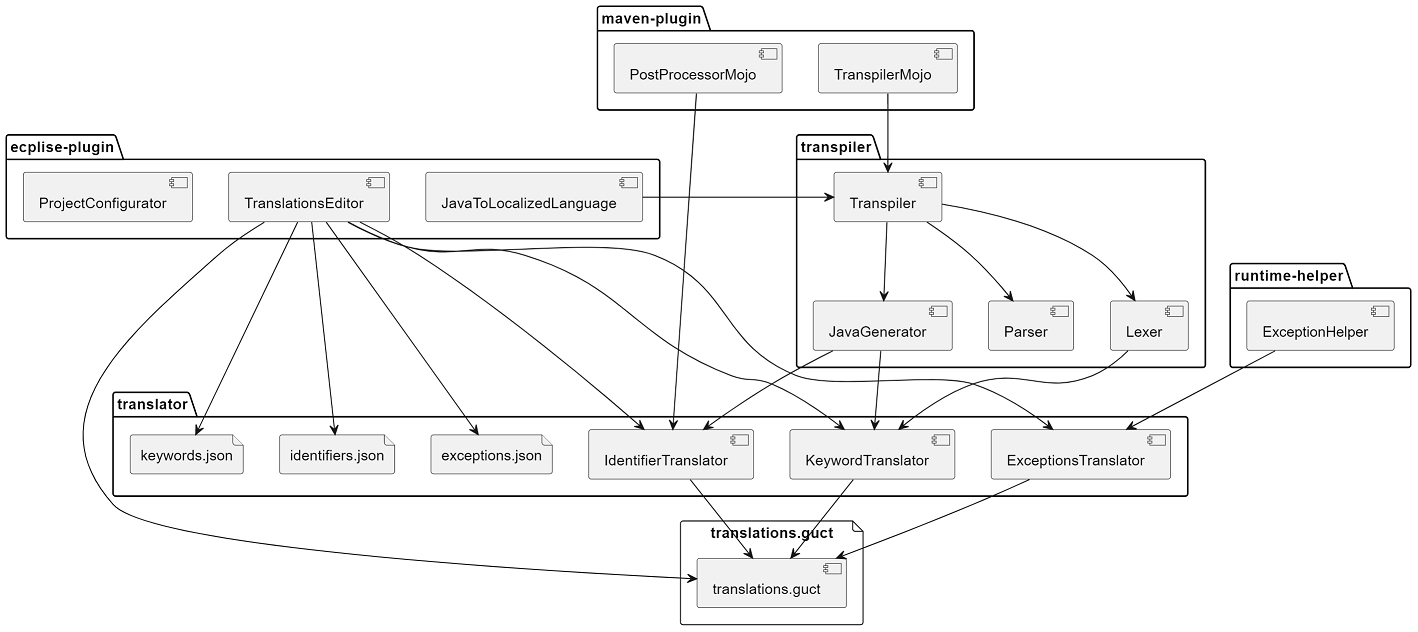
\includegraphics[width=15cm]{ch3-images/components.png}
\caption{Project Components}
\label{fig:Project Components}
\end{figure} 

\section{Implementation Details}
\subsection{Eclipse Plugin}
This plugin adds support for language localization to the Eclipse IDE. 

\subsubsection{Third Party packages}
\begin{enumerate}
    \item \textbf{org.apache.maven.maven-model}: This is a library used to read, parse, and edit the pom.xml file of the user's project.
\end{enumerate}
\subsubsection{Java to Localized Language Command}
This command is added as a context menu item of the project's menu to allow the user to convert an existing Java file or all Java files in a project or a folder depending on the user's selection to a .guc file (or files) depending on the project's default source language. After converting, the java file is backed up to ``.java.bak" and deleted because it can conflict with the generated .guc file during compilation. 

\begin{figure}[H]
\centering
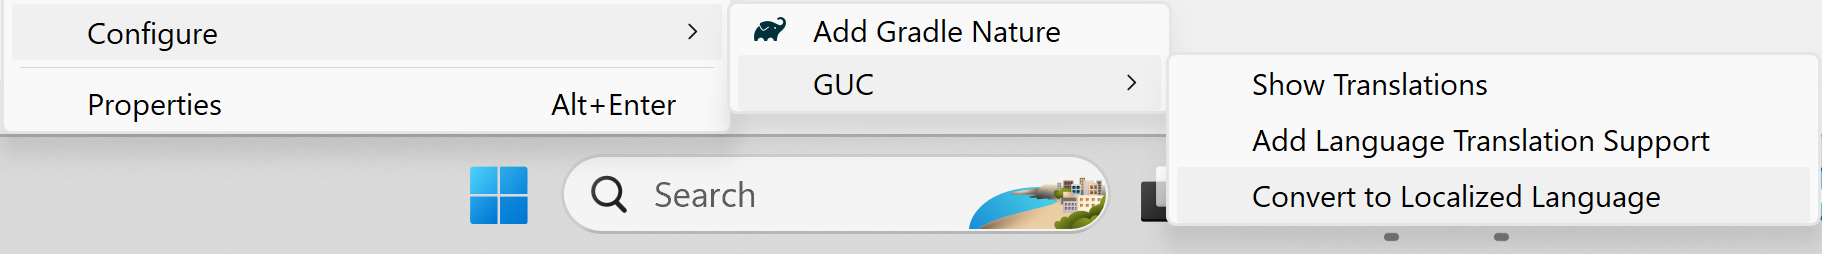
\includegraphics[width=15cm]{ch3-images/eclipsecontextmenu.png}
\caption{Additions to the project's context menu}
\label{fig:Additions to the project's context menu}
\end{figure} 

\subsubsection{Language Translation Support Command}
This command is added as a context menu item of the project's menu to add support for language translation to an existing Maven project. Refer to figure \ref{fig:Additions to the project's context menu} to see the command in the project's context menu. It does so by adding the following changes to the project's pom.xml file:

\begin{enumerate}
    \item Add the repository https://maven.languageslocalization.com/snapshots to both the plugin repositories and repositories. This Maven repository contains my dependencies so that Maven can download the required libraries.
    \item Add the translations.guct as a resource in the output jar file for the project so it could be read by the Runtime Helper package (which will be discussed later) during runtime to perform exceptions translation.
    \item Add the Runtime Helper package as a dependency for the project which is used to translate exceptions in runtime. By referencing this library, all the other needed packages such as the Translator package are included in the project by being indirectly referenced.
    \item Add the build-helper-maven-plugin to make sure that the generated .java files are included in the build.
    \item Add the Transpiler Maven Plugin package to transpile the .guc files and process the .class files after compilation (which will be explained later).
\end{enumerate}

\subsubsection{Translations Editor}
This editor is used to translate keywords, identifiers, and exceptions and saves these translations in the translations.guct file. The editor can be opened by pressing ctrl+G or using the command added in the project menu (see to figure \ref{fig:Additions to the project's context menu}). The translation.guct file has the extension .guct to be a content type to be able to create the user interface for the file. This editor is a Multi-page Editor which consists of five pages:

\begin{enumerate}
    \item \textbf{Keywords Page}: This page is used to translate Java keywords to any target language chosen by the user. The keywords and their translations are represented in a table where the left column is the keyword and the right column is the translation. There is a drop-down menu to select the target language. There is also a button to add default translations without changing the translation already edited by the user, which is disabled if there are no translations to a certain target language. The editor calls the Keyword Translator component (which will be discussed later) to read and write the translations. The following figure shows the Keywords Page in Eclipse:
   
    \begin{figure}[H]
    \centering
    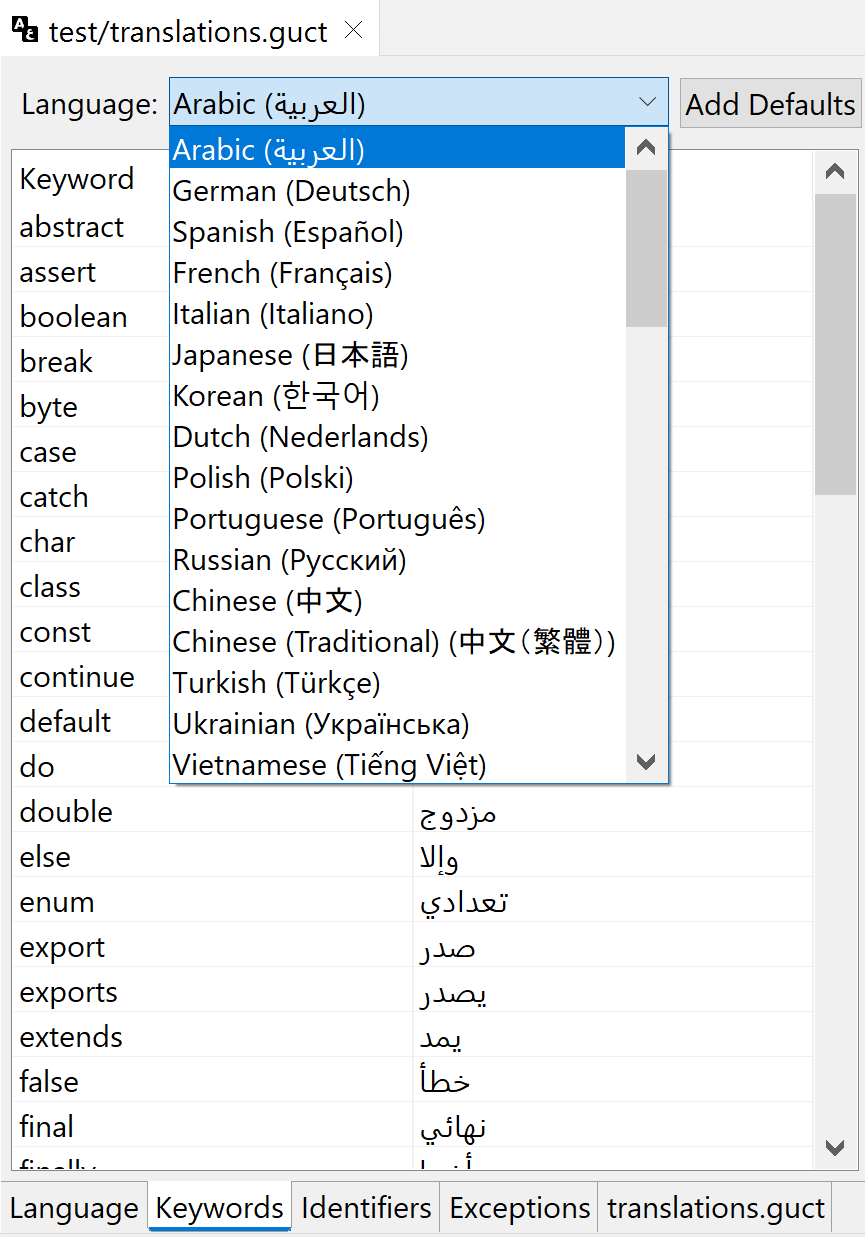
\includegraphics[height=9cm]{ch3-images/keywordspage.png}
    \caption{Translations Editor: Keywords Page}
    \label{fig:Translations Editor: Keywords Page}
    \end{figure}
    
    \item \textbf{Identifiers Page}: This page is used to translate identifiers to any target language chosen by the user. This page is similar to the Keywords Page but has some differences. The identifiers and their translations are represented in a tree instead of a table because Java has many identifiers. This tree is created by traversing the src.zip file found in the Java home folder. Moreover, there is a search bar to search for a specific identifier. Searching can be case-sensitive or exact match or both of them. Translations are performed by calling the Identifier Translator component (which will be discussed later). The following figure shows the Identifiers Page in Eclipse:

    \begin{figure}[H]
    \centering
    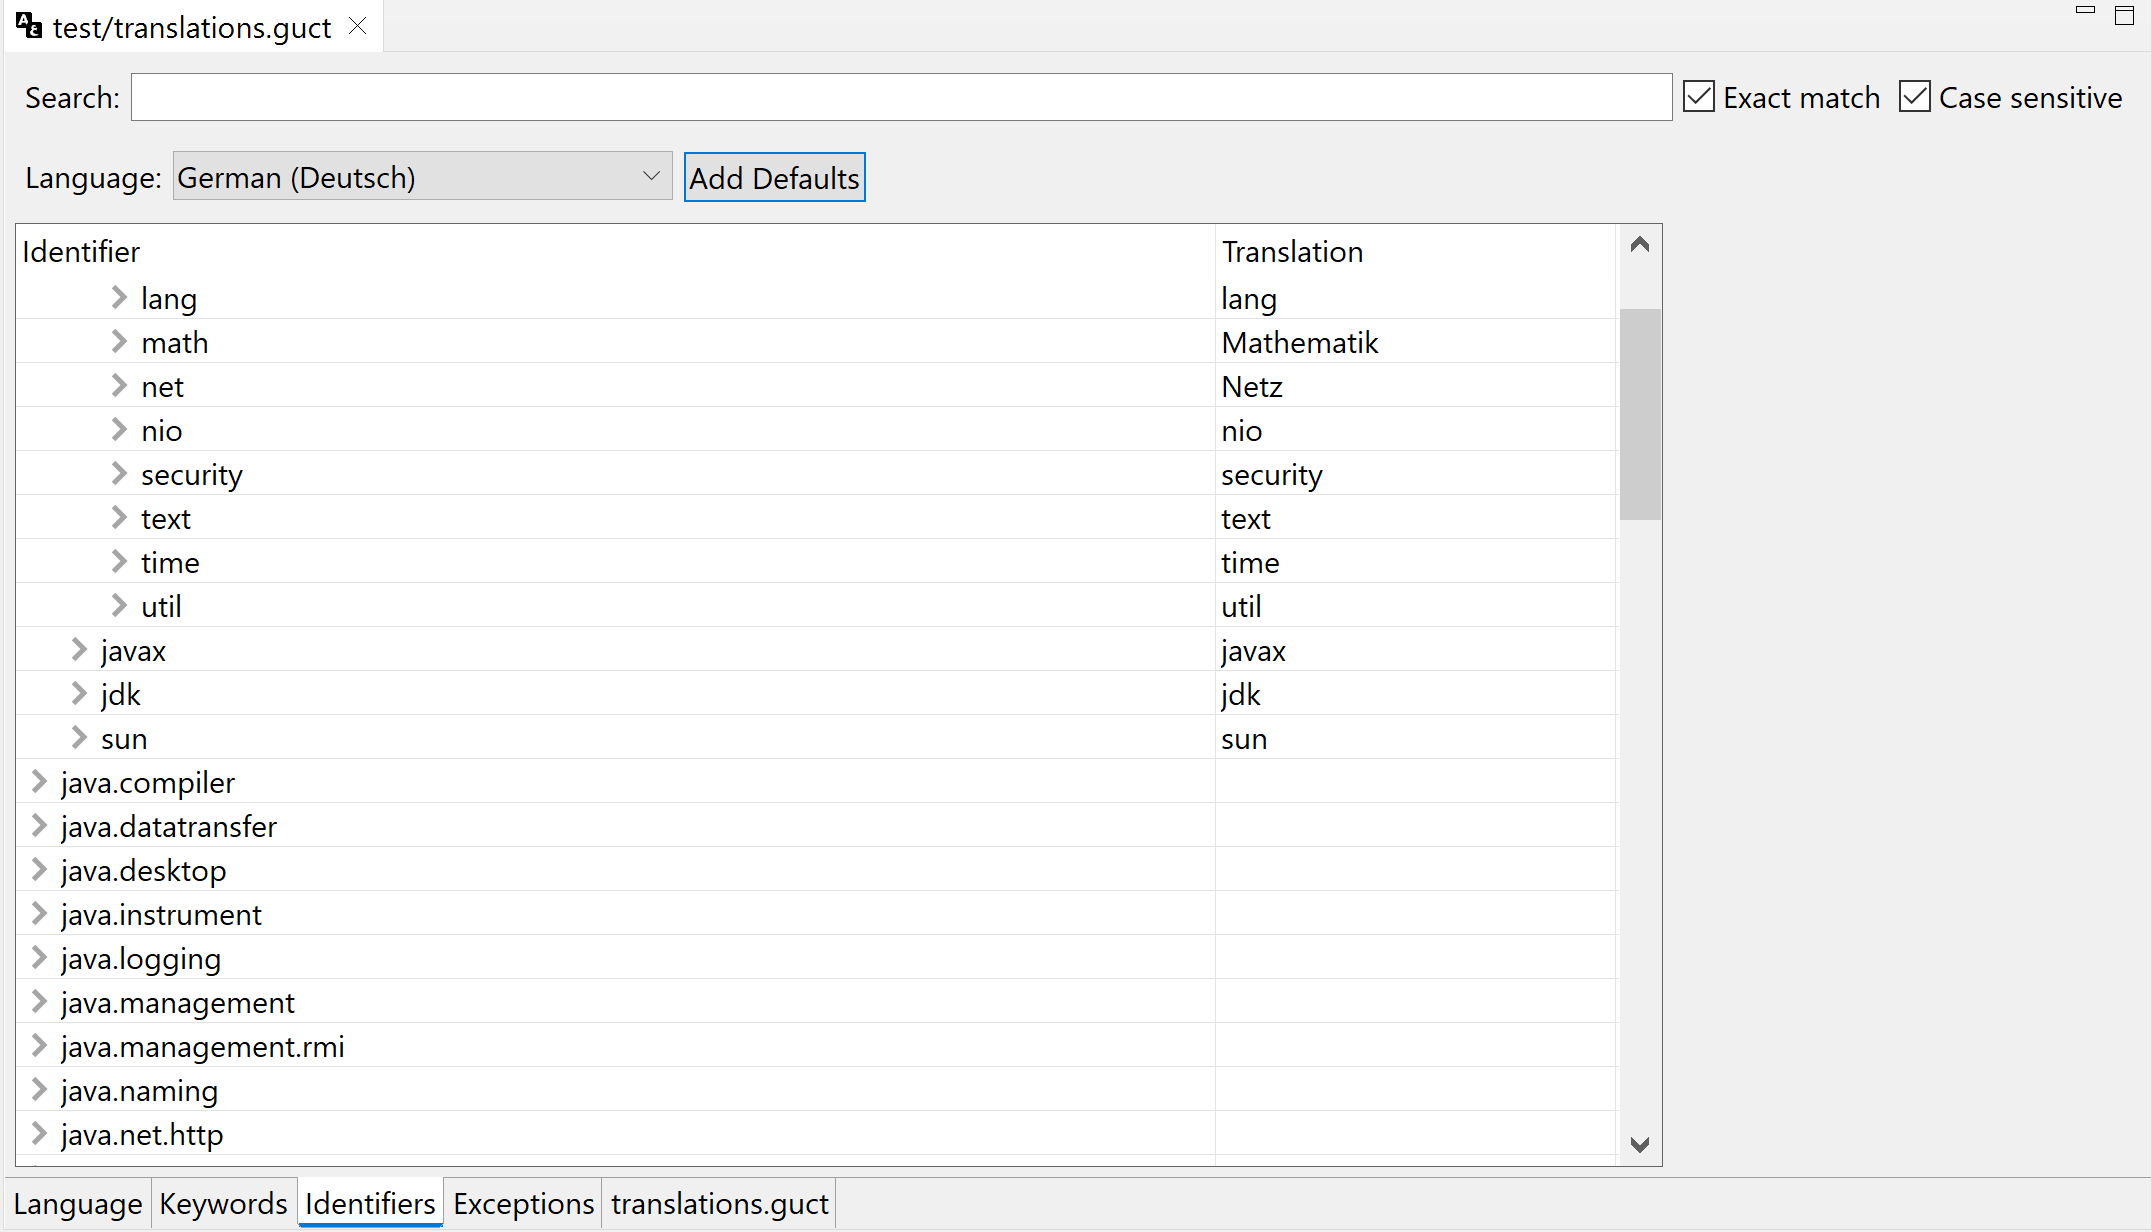
\includegraphics[width=15cm, height=10cm]{ch3-images/identifierspage.png}
    \caption{Translations Editor: Identifiers Page}
    \label{fig:Translations Editor: Identifiers Page}
    \end{figure}
    
    \item \textbf{Exceptions Page}: This page is used to translate exceptions. It is similar to the Identifiers Page but with some differences. One difference is that the tree represents the classes that inherit from the class Throwable instead of representing all classes, methods, and fields. One of the challenges, relating to runtime exception messages translation, is that the message usually includes information that helps the user identify what went wrong. For example, the message "Index 15 out of bounds for length 10" has two pieces of information that can help the user fix the problem. The first is the array index 15, and the second is the array of length 10. The translator extracts those values using Regular Expressions and includes them in the translated message, as explained in this section and later in more detail in the Translations File section. To achieve this, the tree has three columns instead of two. One for the exception names, one for the regex (Regular Expression), and one for the translation of the exception's message. The regex field must be written in English. When a user writes in the regex column, a message is automatically written in the translations field in English, which is a copy of the regex statement except that the capture groups are replaced (which will be discussed later in detail). To translate to another language like Arabic, the user must edit the automatically generated message to Arabic, leaving the symbols replaced with the capture groups. The user can write more than one regex for the same exception, so when they enter a regex statement, another row for the same exception is created. To delete a regex statement, the message must be deleted. The user can also write a message without a regex if the exception doesn't need a regex. The translations are added to the translation.guct file when the user saves all their changes. Note that if the user didn't enter a translation without a regex, a default translation would be automatically written in the translations.guct file (i.e. the default translation will be English (Java)). The following figure shows the Exceptions Page in Eclipse:

    \begin{figure}[H]
    \centering
    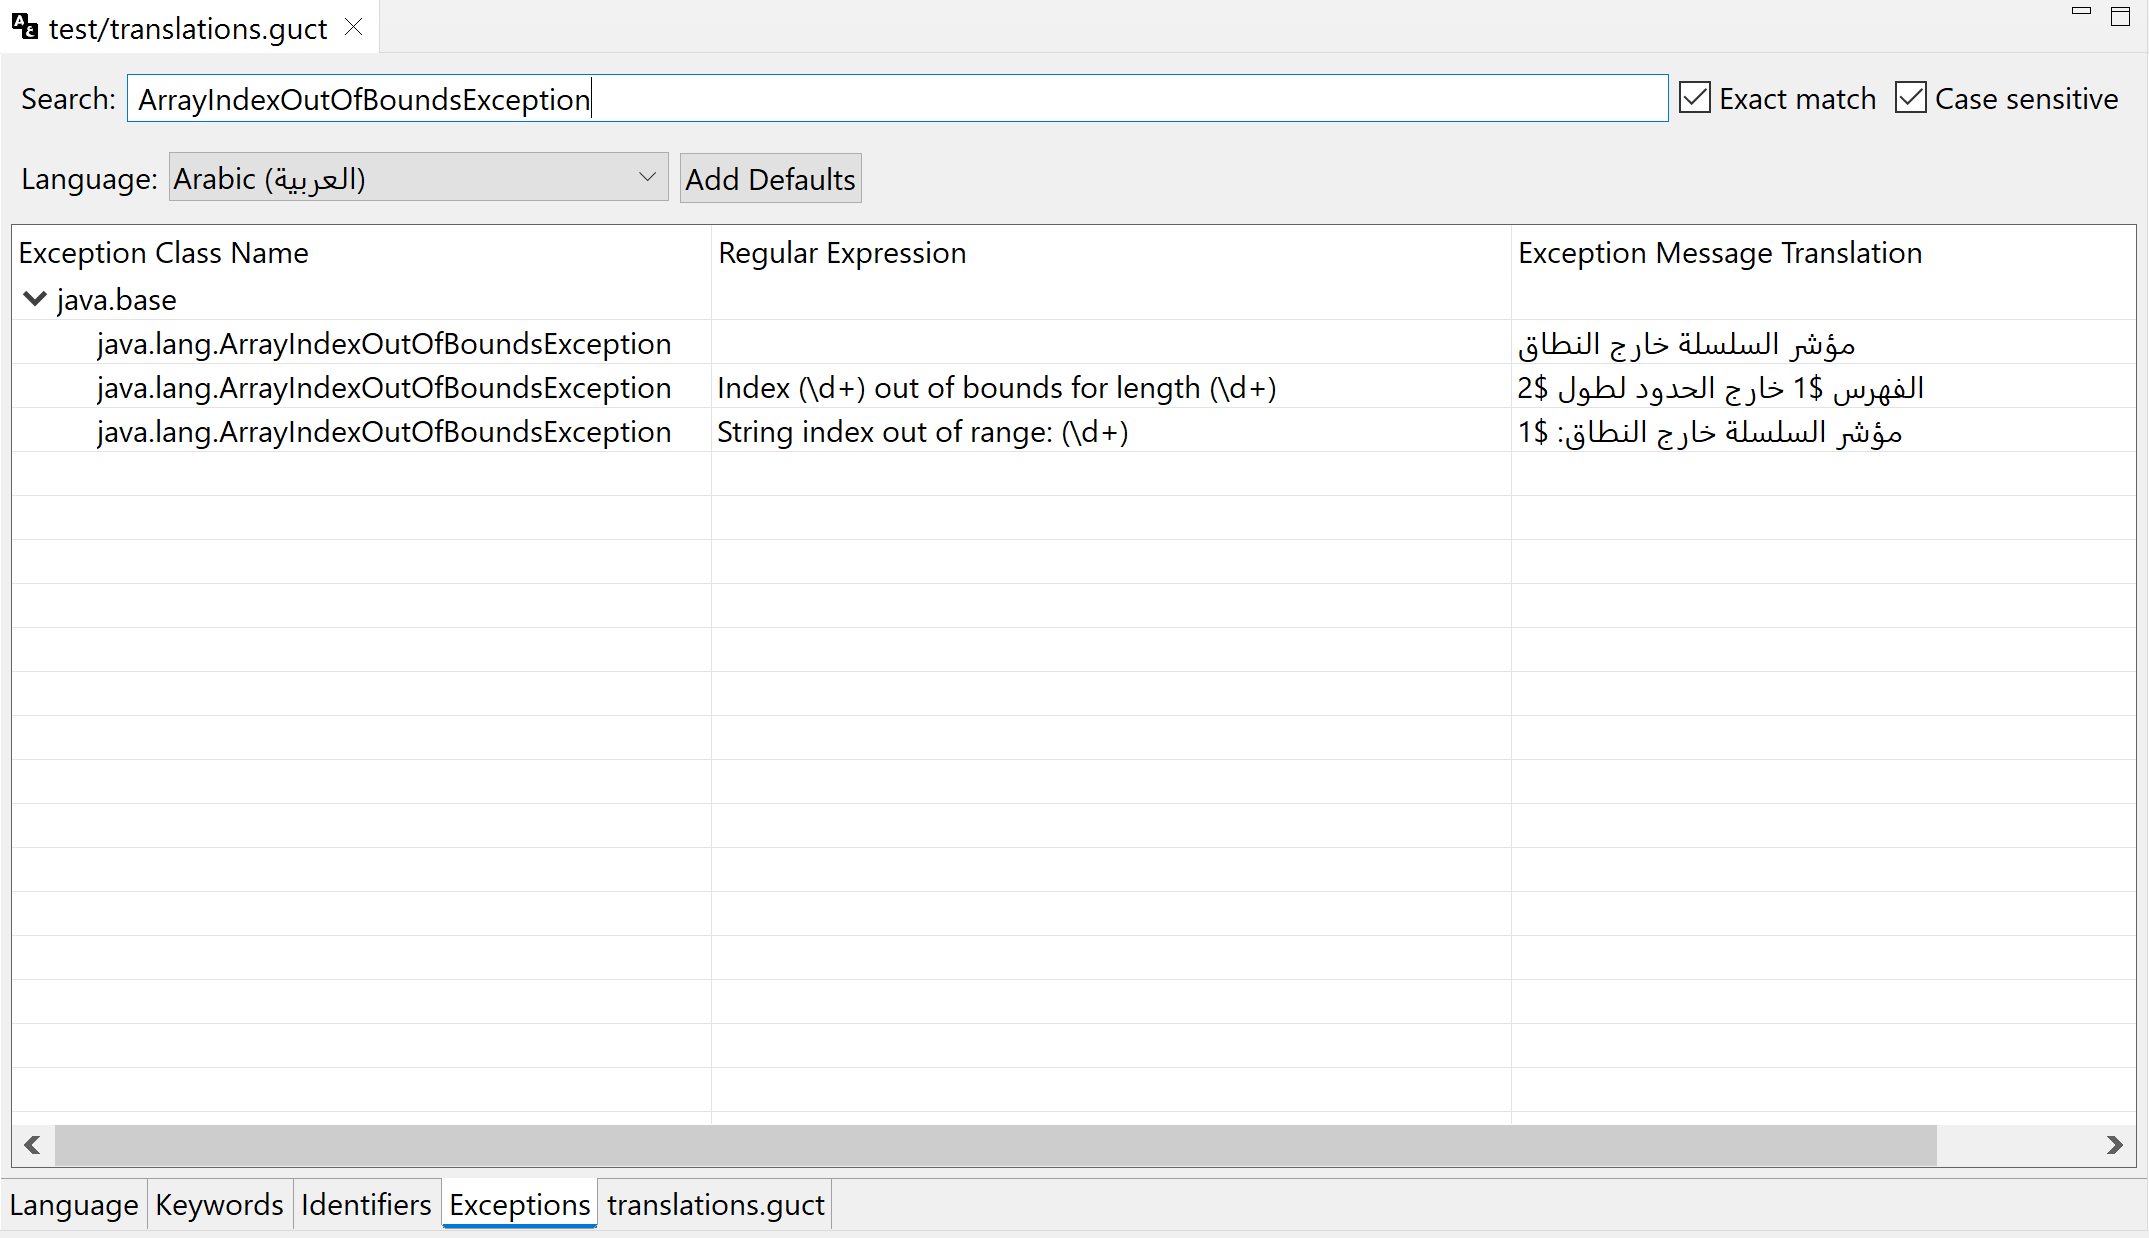
\includegraphics[width=15cm, height=10cm]{ch3-images/exceptionspage.png}
    \caption{Translations Editor: Exceptions Page}
    \label{fig:Translations Editor: Exceptions Page}
    \end{figure}

    
    \item \textbf{Project Language Page}: On this page, the user can change the default language of the project. The default language is initially set to Arabic. Languages are represented in a drop-down menu. The following figure shows the Project Language Page in Eclipse:
    
    \begin{figure}[H]
    \centering
    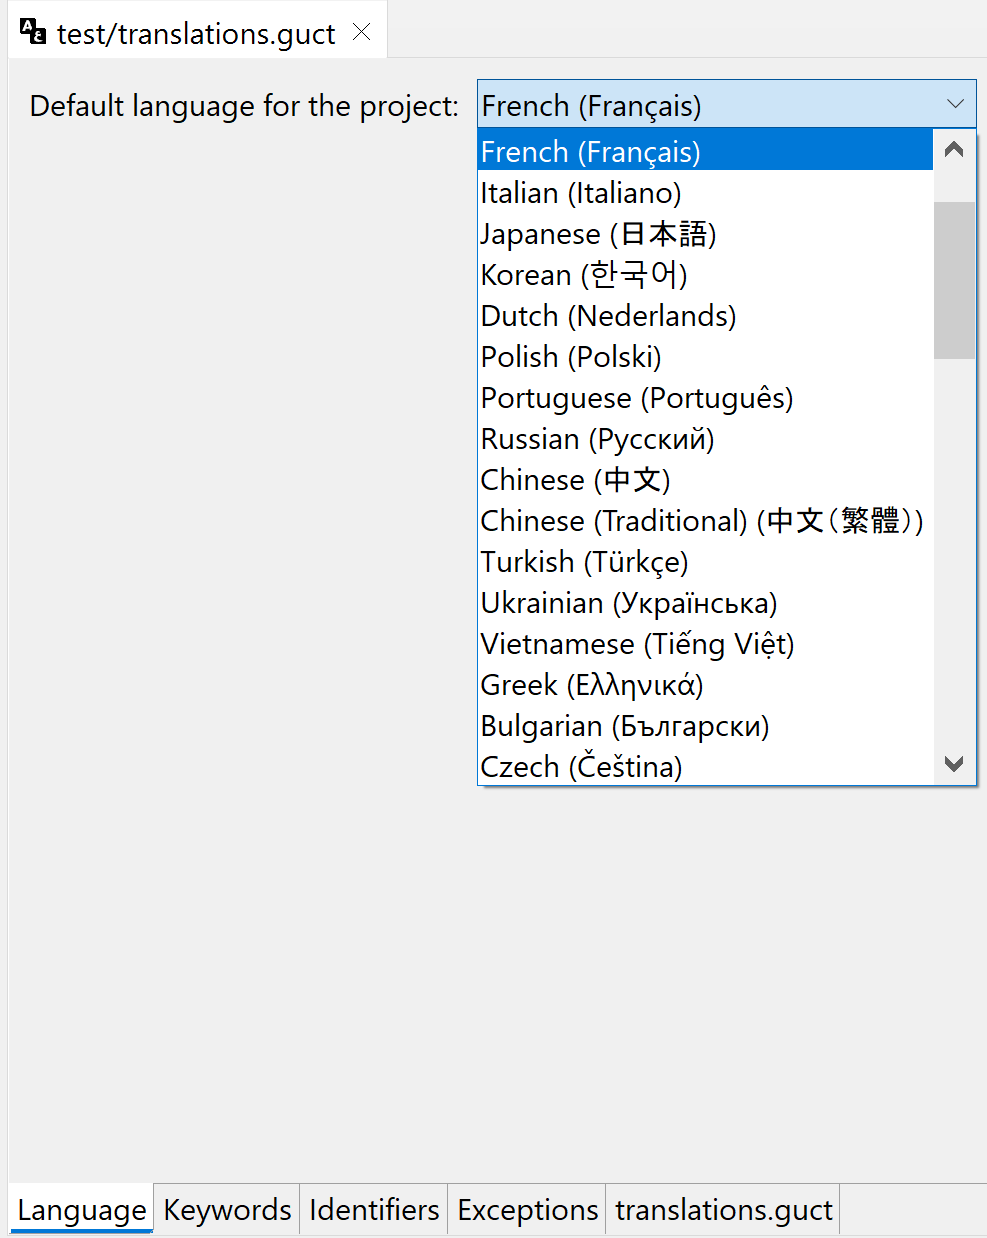
\includegraphics[width=10cm, height=10cm]{ch3-images/defaultlanguage.png}
    \caption{Translations Editor: Project Language Page}
    \label{fig:Translations Editor: Project Language Page}
    \end{figure}

    \item \textbf{translations.guct}: This page is used to translate keywords, identifiers, and exceptions and change the project language by editing the JSON directly. This makes it easier for the user to add translations if they have a JSON file filled with translations. The updates done to JSON are reflected in the user interface of the other pages and vice versa.

\end{enumerate}

\subsubsection{Source-code Editor}
This editor is used to write the programs based on the chosen project language. It has only one page, and the file has an extension ``.guc" to be a content type in Eclipse. The editor supports bidirectional languages like Arabic, Urdu, and Persian. The following figures show the Bubble Sort algorithm in Java and its equivalent Arabic code after using the ``Convert to Localized Language" command (see figure \ref{fig:Additions to the project's context menu}): 

    \begin{figure}[H]
    \centering
    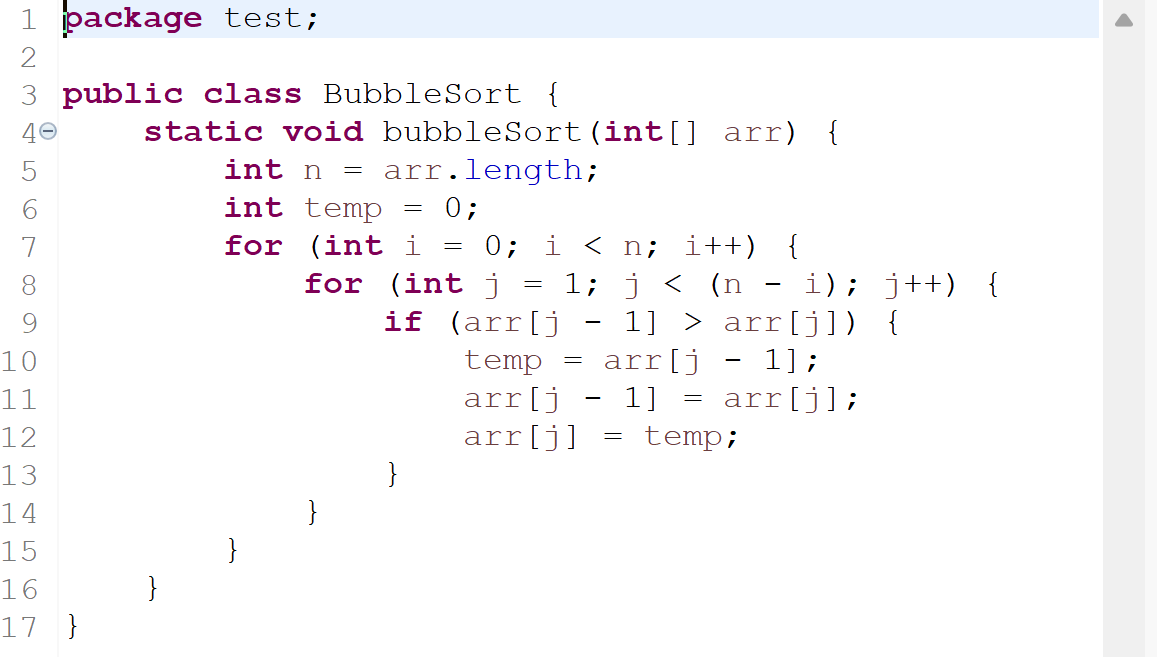
\includegraphics[width=6.5cm]{ch3-images/bubblesort.png}
    \caption{Bubble Sort Algorithm in Java}
    \label{fig:Bubble Sort Algorithm in Java}
    \end{figure}

    \begin{figure}[H]
    \centering
    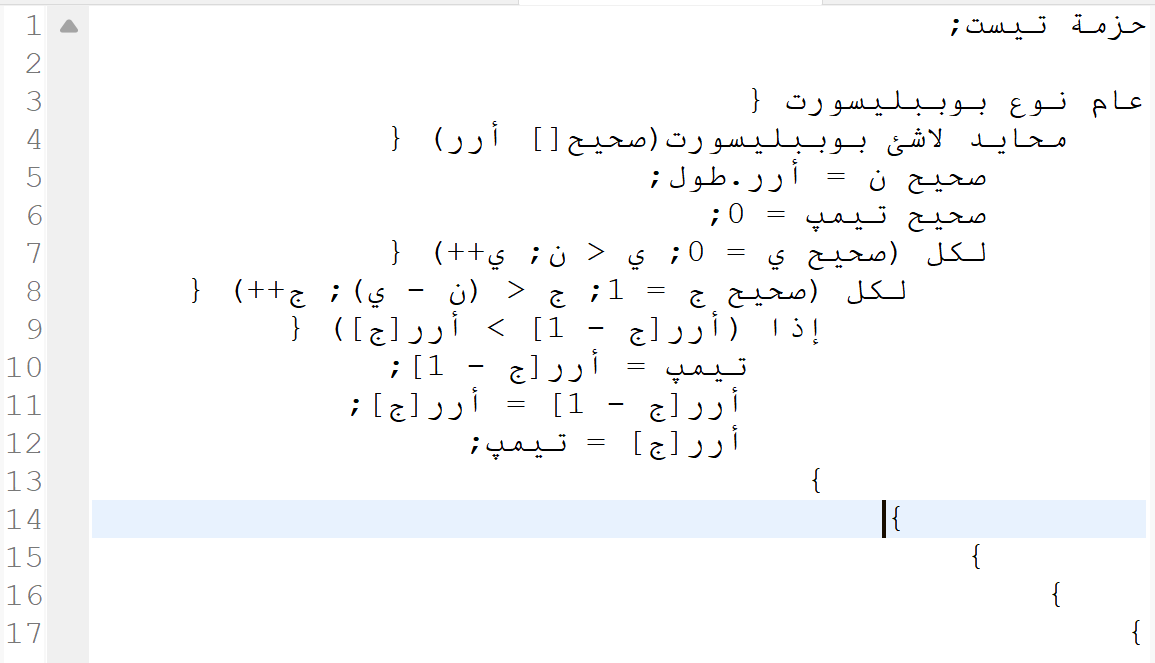
\includegraphics[width=6.5cm]{ch3-images/bubblesort_ar.png}
    \caption{Bubble Sort Algorithm in Arabic}
    \label{fig:Bubble Sort Algorithm in Arabic}
    \end{figure}

The bidirectional support is obvious in the above figure (figure \ref{fig:Bubble Sort Algorithm in Arabic}). In the Transpiler section (which will be discussed later), how the Java code is generated will be explained, taking the Arabic Bubble Sort algorithm as an example.

\subsection{Translations File}
The translations.guct file is one of the main components of the project because its acts like a database in saving information related to translations. The translations.guct file has a structure that is exactly similar to the structure of a JSON file. 

The translation.guct file consists of a JSON object consisting of four keys: defaultLanguage, keywords, identifier, and exceptions. The defaultLanguage key has a value corresponding to the native language that the user will use in their project. This value is the ISO 639-1 of the language name. For example, if the default language is Arabic, then the value will be "ar" and if the user chooses German, then the value will be "de" and so on. The defaultLanguage is initially set to ``ar"" (Arabic) because this project is done in Egypt.

The following key is the keywords key which is a JSON object whose keys are all Java keywords, and values are objects where the key is the ISO 639-1 language name to which the Java keyword is translated and the value is the translation of the keyword. 

The next key is the identifiers and it has exactly the same structure of keywords. Note that if a keyword or identifier is not found, then its translation to any language will be the keyword or the identifier itself. Moreover, when I have a full class name or a package name such as "java.lang.String", it is treated as three separate identifiers java, lang, and String.

The last key is the exceptions key and it includes another object where the key is the full class name of the exception (e.g. java.lang.ArrayIndexOutOfBoundsException) and the value is an array of objects. This array includes one or more objects because an exception may have more than one error message format where each object consists of two keys: regex and messages. The regex (Regular Expression) key is included in the object because some error messages are not static but dynamic. The regular expression is used to determine whether the exception message matches a specific message format in which case the parameters for the message are captured in capture groups, and these groups are used in the string replacement when the message is translated. For example, the error message of ArrayIndexOutOfBoundsException in Java can change depending on the specific context in which the exception is thrown. This exception is generally thrown when a program attempts to access an array element using an index that is out of bounds. For example, if an array has five elements, but a program tries to access the sixth element, then an ArrayIndexOutOfBoundsException will be thrown. The error message displayed when this exception occurs in Java will typically include information about the array that caused the exception, as well as the index that was out of bounds. For example, the error message might look something like this:
\begin{lstlisting}[language=java]
Exception in thread "main" java.lang.ArrayIndexOutOfBoundsException: Index 6 out of bounds for length 5
    at MyClass.myMethod(MyClass.java:25)
    at MyClass.main(MyClass.java:10)

\end{lstlisting}


The regex value should be "Index (\textbackslash{\textbackslash{d+}}) out of bounds for length (\textbackslash{\textbackslash{d+}})" because the 6 and the 5 can be other numbers in other cases. The messages key is the other key in the object and it includes another object which is the ISO 639-1 language name to which the Java keyword is translated and the value is the translation of the keyword. In this example, the translation should include \$1 and \$2 which are replaced by the values of the corresponding capture groups. Note that the regex is an optional key and mustn't be included in the object if the error message is not dynamic. When the regular expression is omitted, the corresponding translation is used when none of the regular expressions match the exception message.

Here is a simple example of a JSON object that could be written in the translations.guct file: 

\begin{figure}[H]
\centering
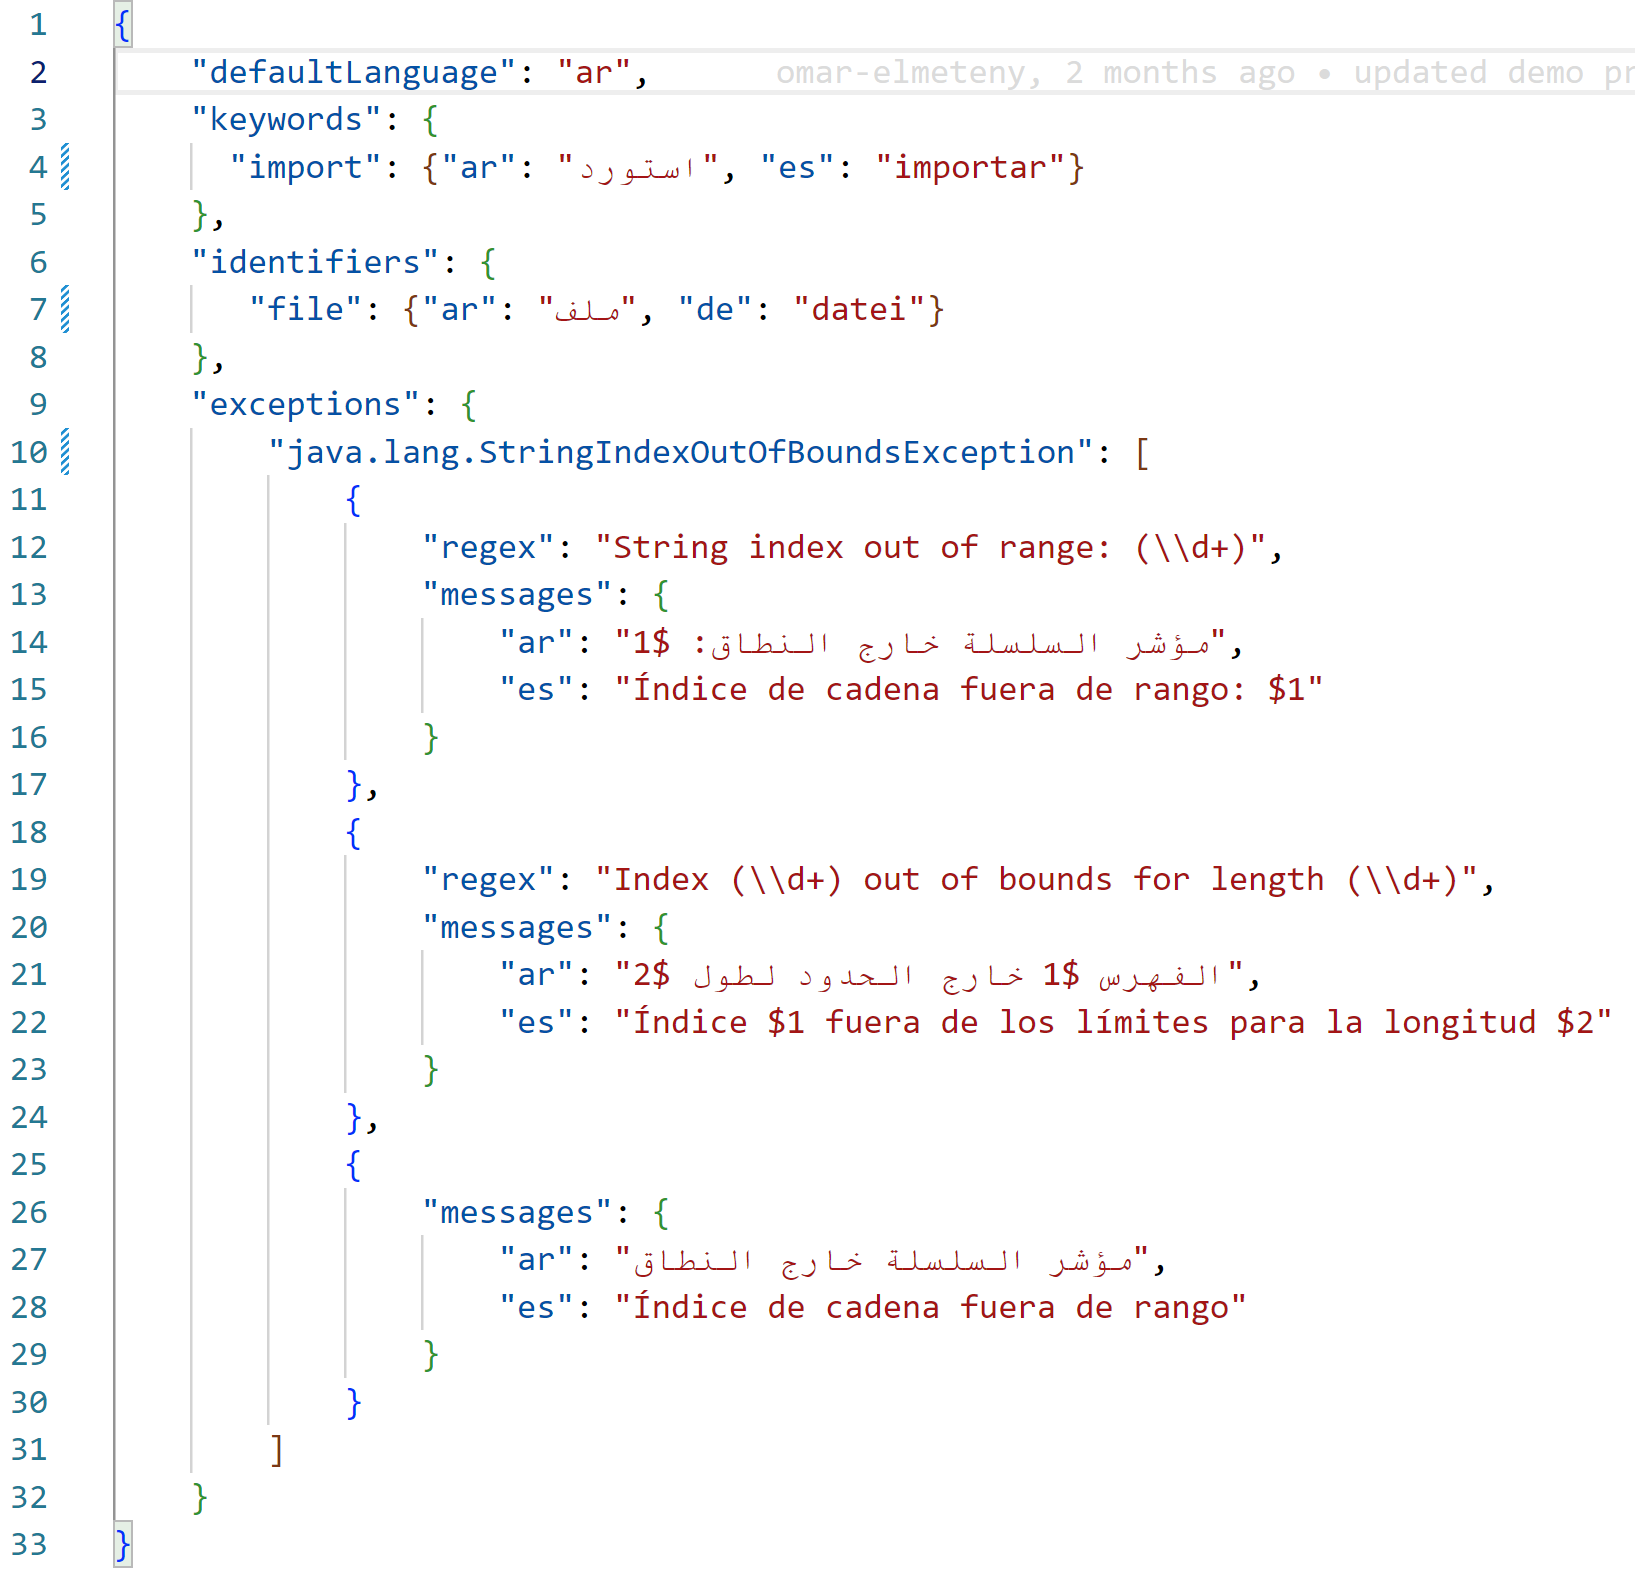
\includegraphics[width=12.5cm]{ch3-images/translationsfile.png}
\caption{An example of a translation.guct file}
\label{fig:An example of a translation.guct file}
\end{figure} 

\subsection{Translator Package}
The Translator package is responsible for translating keywords, identifiers, and exceptions from the source language to English and vice versa. This is done by reading the JSON file.
\subsubsection{Third Party packages}
The Translator package uses three third-party packages:
\begin{enumerate}
    \item \textbf{org.json}: A package for parsing and writing JSON format.
    \item \textbf{com.ibm.icu.icu4j}: A package to transliterate text using non-ASCII letters to ASCII letters. For example ``\<زر>" is transliterated to ``zr".
    \item \textbf{commons-io}: Used to handle files containing Unicode Byte Order Marks (BOM).
\end{enumerate}

\subsubsection{Resource Files}
The Translator package contains three JSON files including default translations for keywords, identifiers, and exceptions. The translations don't cover all languages but only five languages: Arabic, French, German, Italian, and Spanish because these are the most commonly spoken languages.
\begin{enumerate}
    \item \textbf{keywords.json}: This file contains the default translations for all Java keywords.
    \item \textbf{identifiers.json}: This file contains the default translations for Java's most commonly used identifiers (e.g. String).
    \item \textbf{exceptions.json}: This file contains the default translations for Java's most commonly thrown exceptions (e.g. ArrayIndexOutOfBoundsException).
\end{enumerate}
Note that the structure of each file is exactly similar to its corresponding key in the translations.guct file.

\subsubsection{Keyword Translator}
The Keyword Translator is responsible for loading the keyword translations from JSON format (see translations.guct above) to memory. It is used in translating a keyword from Java to a target language and from a source language to Java. Moreover, it is used to determine whether a particular keyword has a translation to any native language or not. It also has an API to add/change keyword translations used by the Eclipse Plugin for editing translations (as discussed earlier). The Keyword Translator can convert the data back to JSON to be saved to the project's translations.guct file.
\subsubsection{Identifier Translator}
The Identifier Translator works in a similar manner to the Keyword Translator. However, the difference is that if an identifier doesn't have a translation to the target language and both source and target languages use different scripts (e.g. Arabic and Latin), the Identifier Translator will transliterate the identifier to the target language's script (e.g. ``\<زر>" is transliterated to ``zr").
\subsubsection{Exception Translator}
The Exception Translator is used to translate exception messages and other identifiers that appear in the stack trace. It uses the Identifier Translator to translate the identifiers that appear in the stack trace. The Exception translator works only at runtime because this is when the exceptions are thrown.
\subsection{Runtime Helper Package}
This package has helper methods that are called by the generated Java code during runtime. 
\subsubsection{Third Party packages}
\begin{enumerate}
    \item \textbf{org.ow2.asm}: This library reads the .class files which are executed by the \ac{JVM} to read information about the identifiers that were translated during the transpilation process.
\end{enumerate}
\subsubsection{Exception Helper}
This component performs the task of translating the exception messages and the stack trace of the thrown exceptions. It uses the Exception Translator component in the Translator package to perform these tasks. It reads the translations.guct file during runtime (via the Translator package) and also reads the information about the identifiers that were translated during the transpilation process. This information is written in the class file by the PostProcessorMojo component (which will be explained later).
\subsection{Transpiler Package}
This package performs the actual transpilation of code from the source language to Java and vice versa. 
\subsubsection{Third Party packages}
\begin{enumerate}
    \item \textbf{org.antlr.antlr4-runtime}: \ac{ANTLR} \cite{antlr} is a powerful parser generator for reading, processing, executing, or translating structured text or binary files. This package provides the core functionality for the lexer and parser.
    \item \textbf{antlr/grammars-v4}: This is an open source repository containing ANTLR4 grammar files for many programming languages including Java. I used the Java9 grammar files from this repository and made some modifications in order to make it work with the source languages. 
    \item \textbf{org.antlr.antlr4-maven-plugin}: This is a maven plugin used to generate Java source code files from antlr grammar files.
    \item \textbf{org.codehaus.mojo.build-helper-maven-plugin}: This is a maven plugin used to make maven include the generated Java files in the build. 
\end{enumerate}
\subsubsection{Lexer}
The lexer is a Java class generated by ANTLR from the lexer grammar file obtained from antlr/grammars-v4. The original grammar files had the Java keywords hard-coded in the lexer grammar file itself. In order to avoid making many grammar files for all languages, I modified the base class of the generated Java Lexer class in order to have a source language property, and use the Keyword Translator component to translate keywords.

For example, a keyword defined in the original grammar file looks like this:
\begin{lstlisting}
    ABSTRACT: 'abstract';
\end{lstlisting}

In the modified grammar file, the keyword definition calls the CheckKeyword method in the base class rather than having it hard-coded. The CheckKeyword calls checks the sourceLanguage property and calls the Keyword Translator component to translate the keyword before checking if the token matches the keywords.
\begin{lstlisting}
    ABSTRACT : { CheckKeyword("abstract") }? .;
\end{lstlisting}

\subsubsection{Parser}
The parser is a Java class generated by ANTLR from the parser grammar file obtained from antlr/grammars-v4. The original parser grammar file also had the keywords hard-coded. I changed that to reference the lexer's rule names instead. 
Also, the ANTLR lexer grammar rules didn't allow the null literal and boolean literals (true and false) to be treated as lexer rules because they were dynamic, so I moved the rules from the lexer grammar file to the parser grammar file. 

\subsubsection{Java Generator}
The java generator implements the visitor design pattern and inherits the Visitor class generated by ANTLR. It accepts a parse tree generated by the parser after parsing the source file and simplifies the traversal of the parse tree. The core code generation functionality is done by the visitTerminal method which is overridden to check if the terminal node is a keyword or an identifier in which case the Translator package is used to translate them, otherwise the terminal node is written as in the transpiled code. 

Java has two types of exceptions: Checked Exceptions and Unchecked Exceptions. To handle Unchecked Exceptions, I override the visitBlockStatements method to surround the block with a try/catch which catches only RuntimeException and calls the Exception Helper component to translate the exception and its stack trace in the catch block and re-throw the translated exception. For example: 

\begin{figure}[H]
\centering
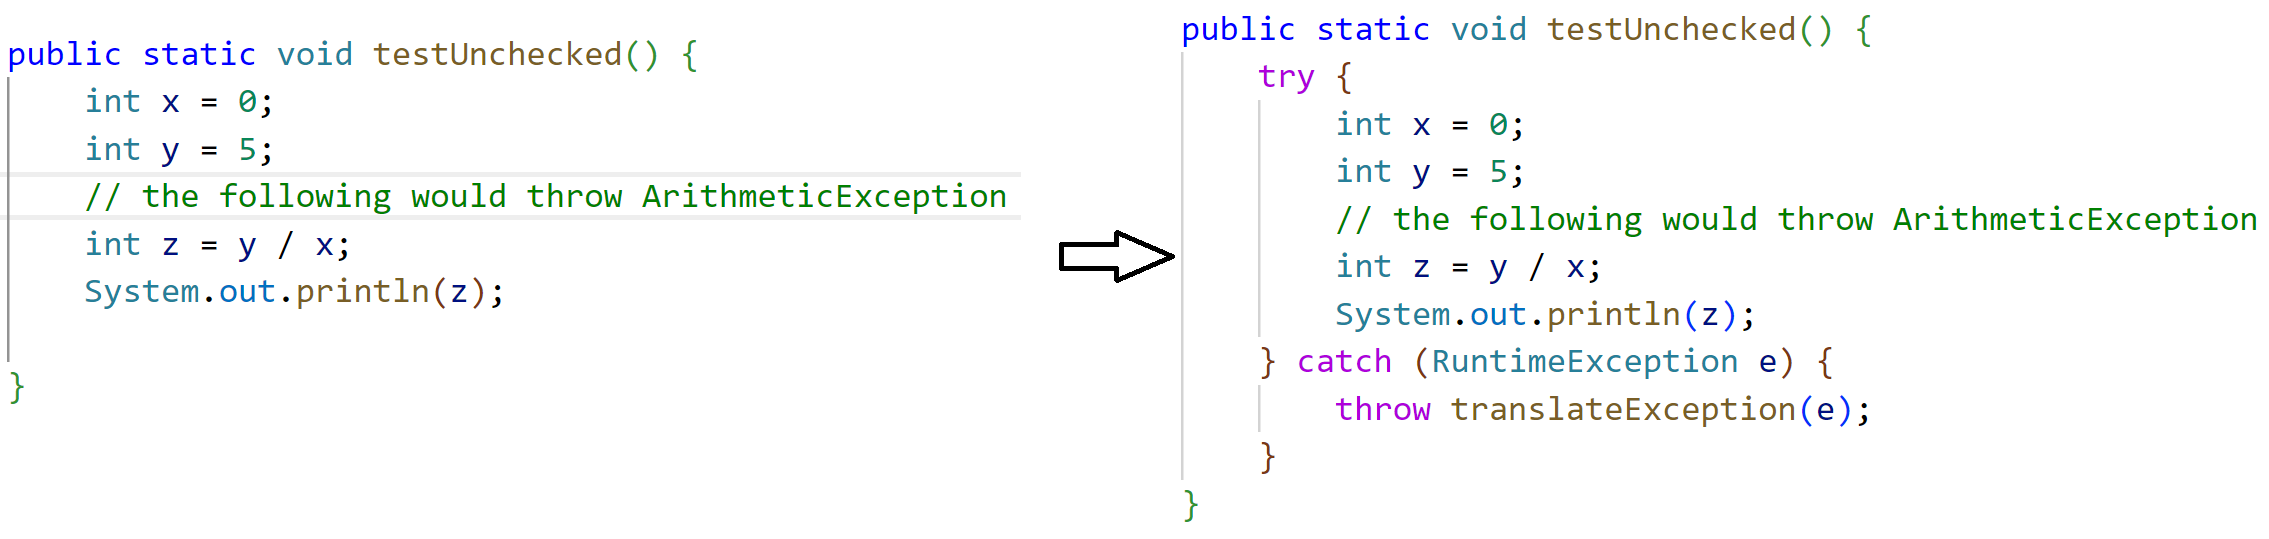
\includegraphics[width=15cm]{ch3-images/unchecked.png}
\caption{An example of a generated code for Unchecked Exceptions}
\label{fig:An example of a generated code for Unchecked Exceptions}
\end{figure} 

To handle Checked Exceptions, I override the visitMethodDeclaration and visitConstructorDeclaration to determine the types of exceptions being thrown and then surround the body of the method or the constructor with try/catch and catch only those exceptions and perform the translation as done with the Unchecked Exceptions. For example:

\begin{figure}[H]
\centering
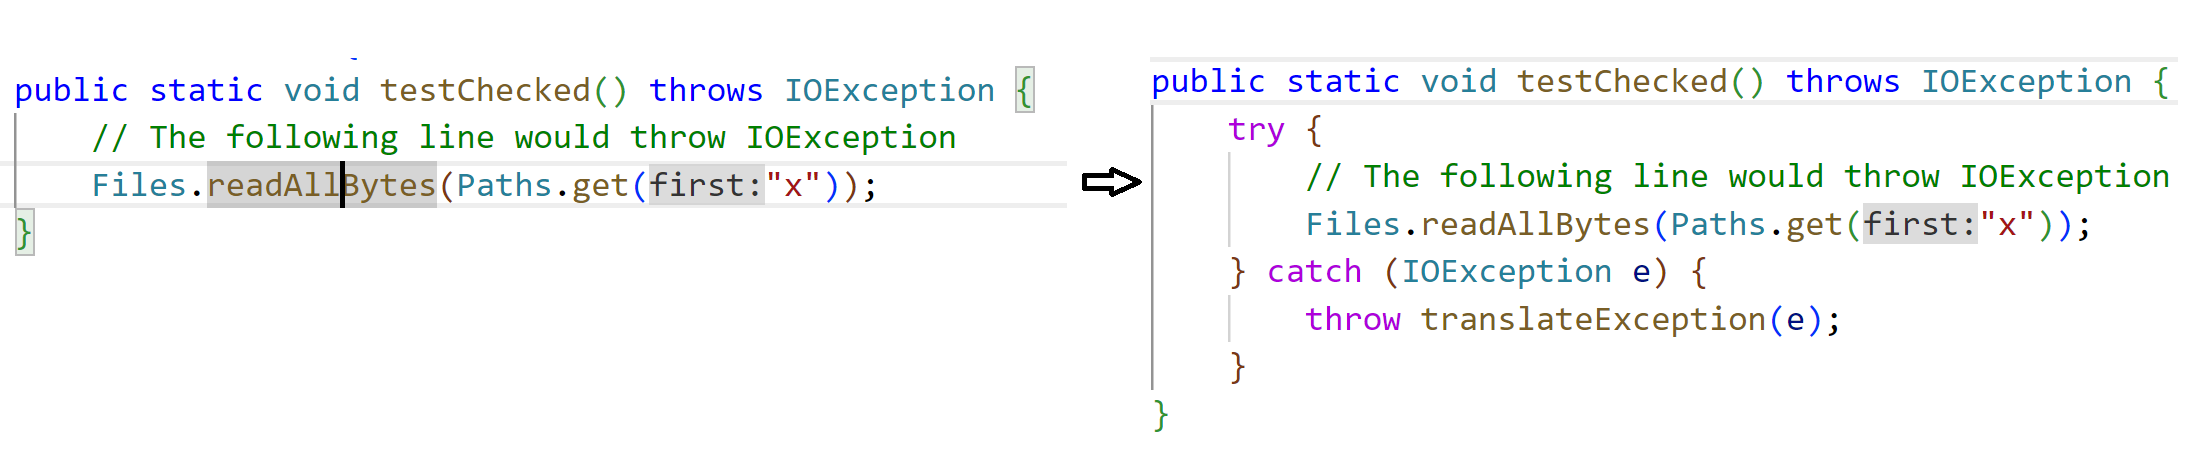
\includegraphics[width=15cm]{ch3-images/checked.png}
\caption{An example of a generated code for Checked Exceptions that is not Caught}
\label{fig:An example of a generated code for Checked Exceptions that is not Caught}
\end{figure} 

Moreover, I override visitCatchClause and visitVariableDeclaratorId to create a new exception variable in the catch block which has the exception translated by the Exception Helper. This is done when the block is already surrounded by a try/catch statement. For Example:

\begin{figure}[H]
\centering
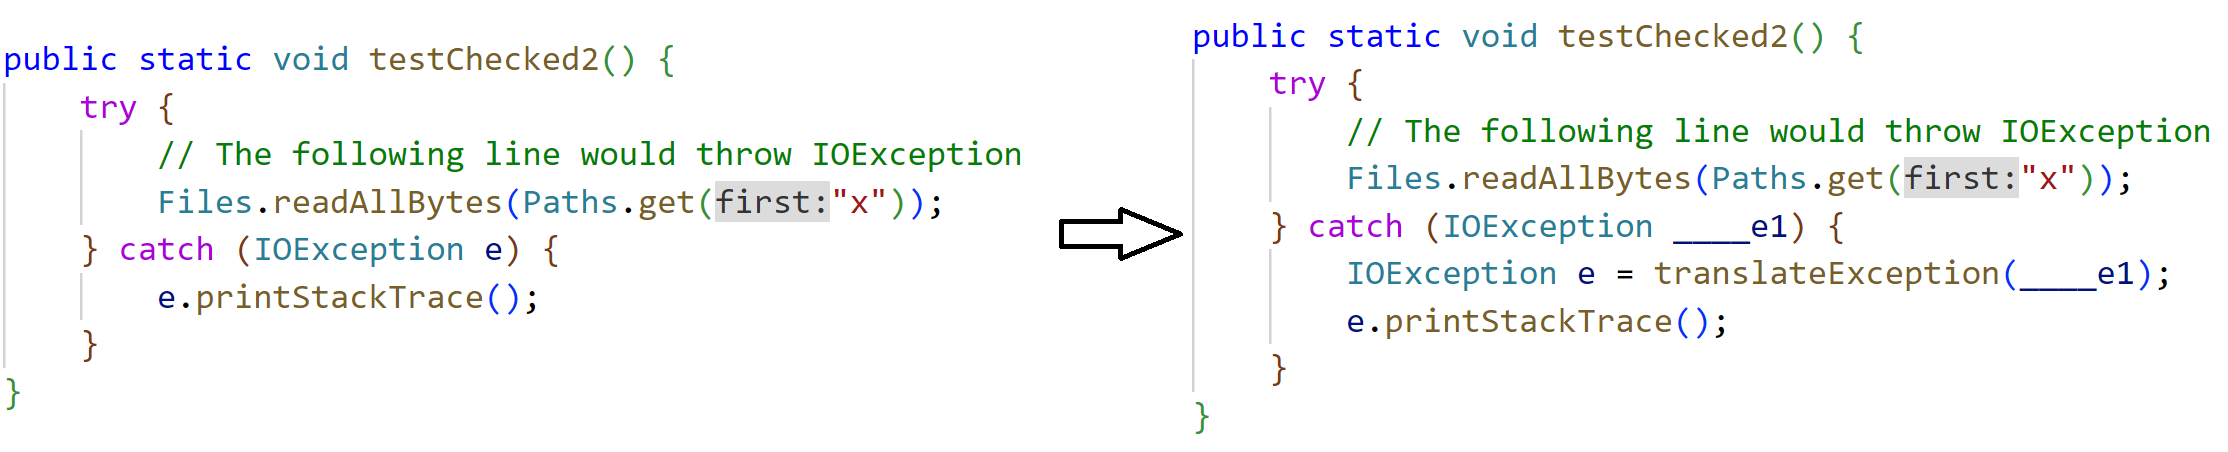
\includegraphics[width=15cm]{ch3-images/checked2.png}
\caption{An example of a generated code for Checked Exceptions that is already Caught}
\label{fig:An example of a generated code for Checked Exceptions that is already Caught}
\end{figure} 

If there is an uncaught exception in the program, Java would call printStackTrace method and then terminates the program. The printStackTrace provided by the Java runtime would print the stack trace and exception class name in English, so I use the visitMethodDeclaration to surround the main method with a try/catch that calls my own implementation of printStackTrace in the Exception Helper component.
\subsubsection{Transpiler}
The Transpiler is used to read the source code file, then calls the lexer to produce the tokens, then calls the parser to generate the parse tree, then finally the java generator traverses the tree to generate the code. It can optionally generate a source map file that maps the line numbers in the source files to those in the target file. It can also optionally generate a JSON file containing all the translated identifiers. This file is embedded after compilation by the PostProcessorMojo (which will be discussed later) so it can be used in runtime to translate exceptions (as explained earlier in the Exception Helper section).

The Transpiler works based on some transpiler options. These options are source language, target language, source encoding, target encoding, the translations object (loaded from translations.guct file), and whether to generate identifiers dictionary or source maps.

Here is an example of the Bubble Sort algorithm transpiled Java code where the source language is Arabic (see figure \ref{fig:Bubble Sort Algorithm in Arabic}):

\begin{figure}[H]
\centering
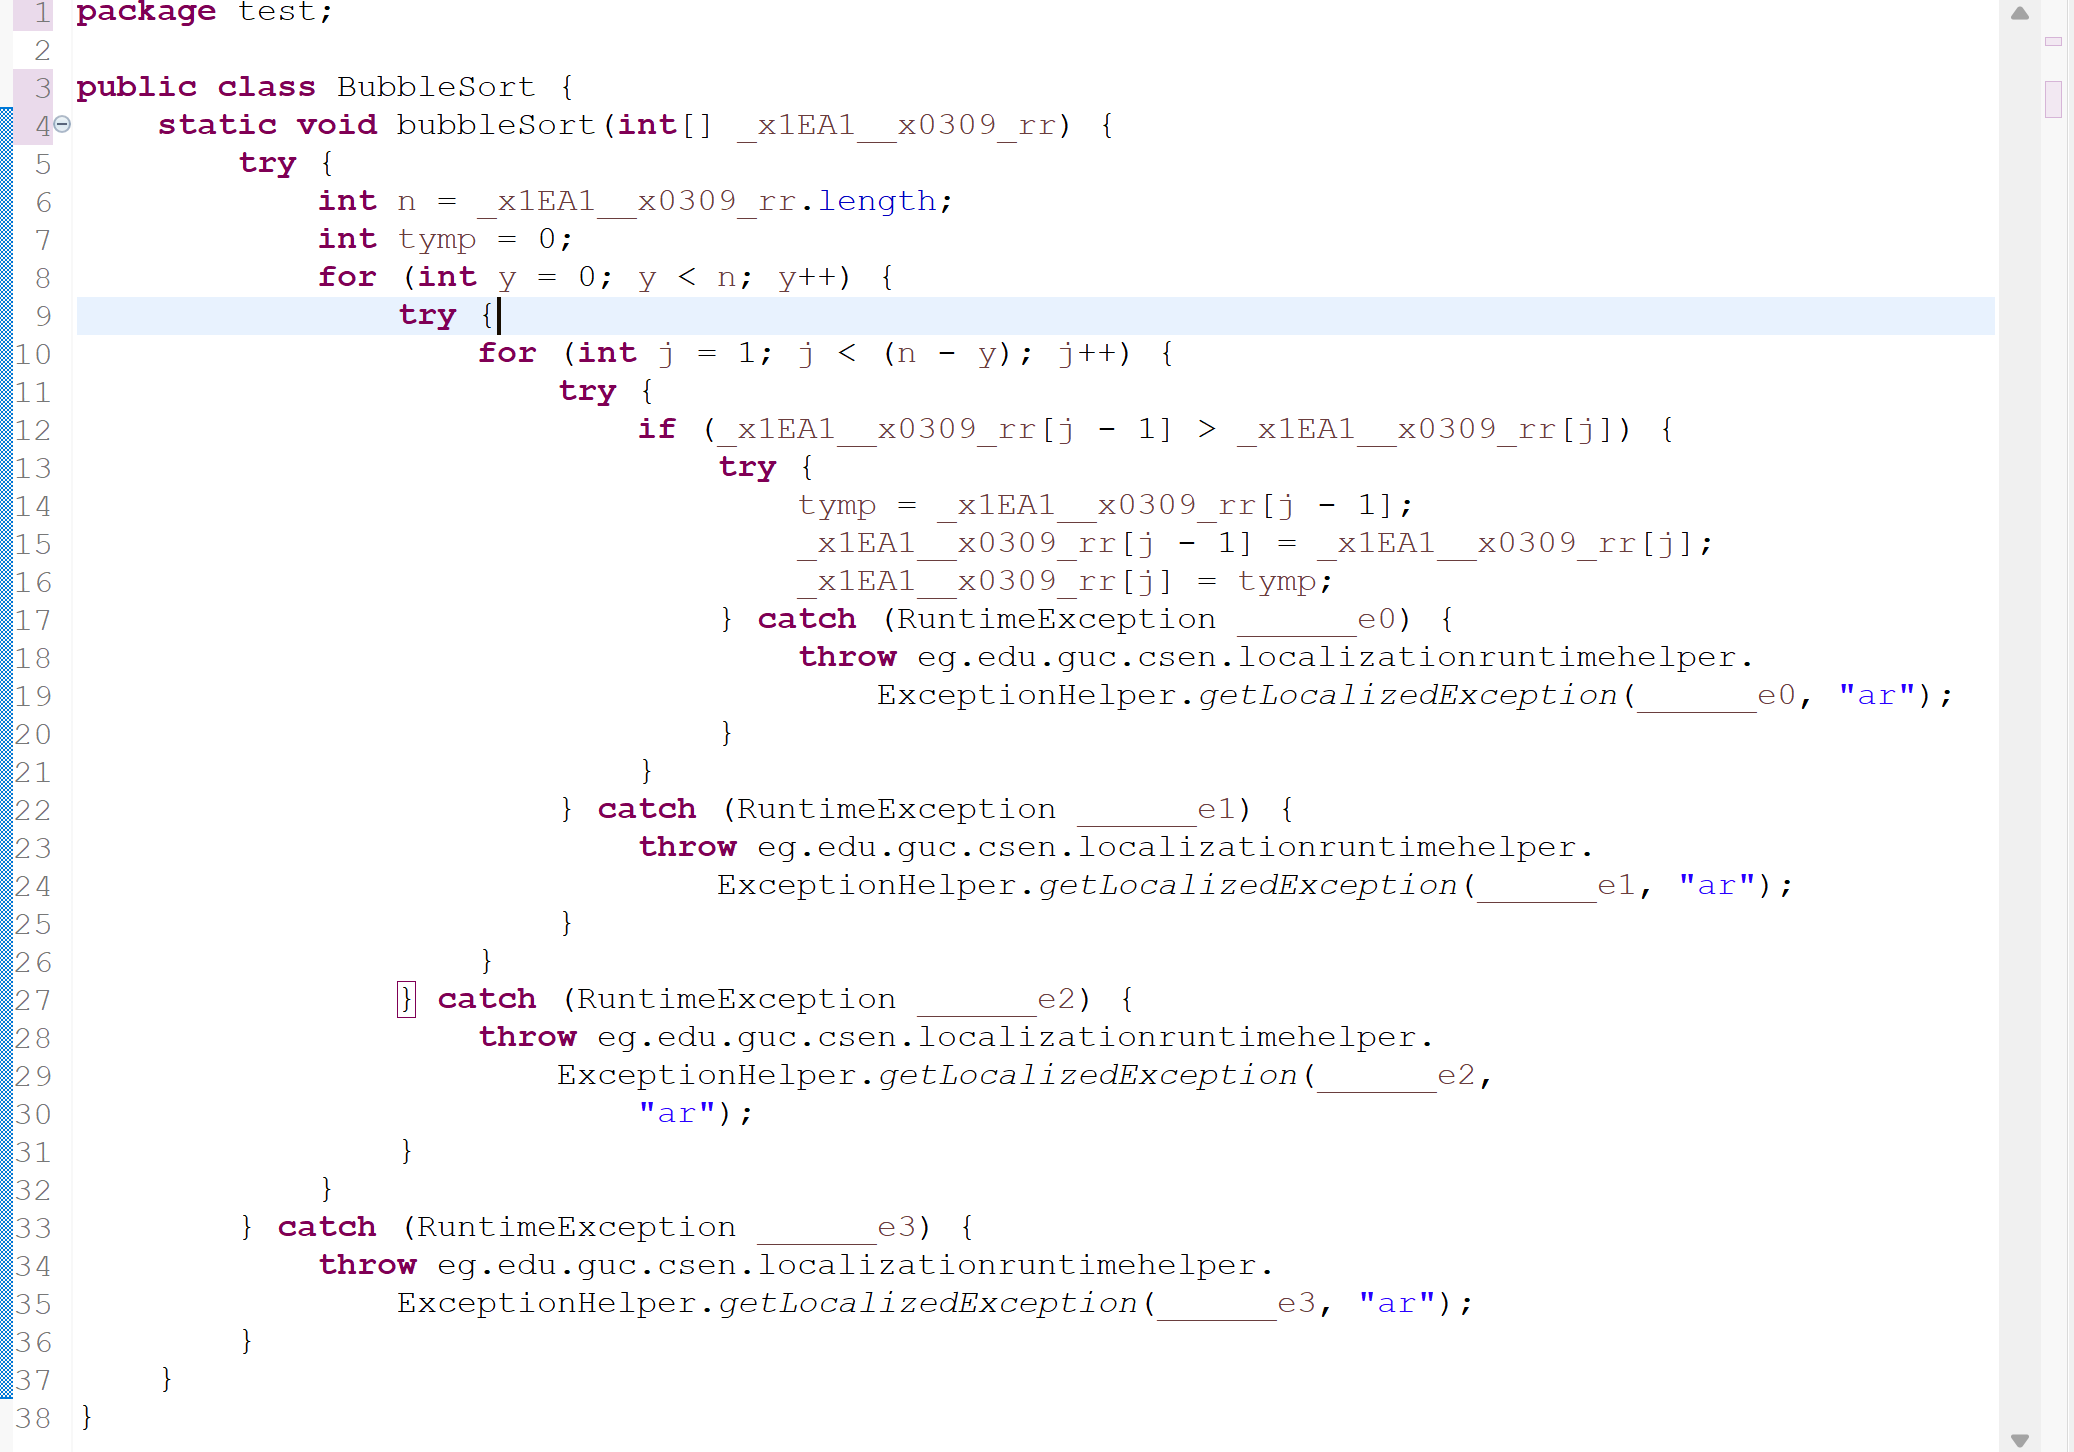
\includegraphics[width=10cm]{ch3-images/bubblesort_transpiled.png}
\caption{The Bubble Sort Algorithm after transpilation}
\label{fig:The Bubble Sort Algorithm after transpilation}
\end{figure} 

\subsection{Maven Plugin Package}
This package is a Maven Plugin that introduces a transpilation step and a post-processing step in the Maven build cycle of the user's project.

\begin{figure}[H]
\centering
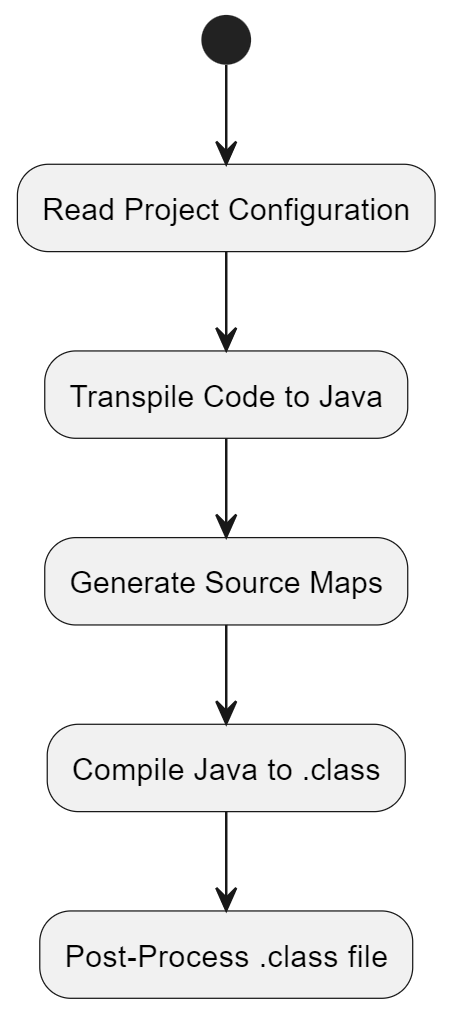
\includegraphics[height=8cm]{ch3-images/compilation.png}
\caption{Compilation flowchart}
\label{fig:Compilation flowchart}
\end{figure} 

\subsubsection{Third Party packages}
\begin{enumerate}
    \item \textbf{org.apache.maven.maven-plugin-api}: It contains a base class for Mojos. A Mojo is an executable goal that runs during the maven build cycle.
    \item \textbf{org.apache.maven.plugin-tools.maven-plugin-annotations}: This library provides annotations to mark fields in a Mojo Class as parameters that can be read from the Maven project file (pom.xml).
    \item \textbf{org.apache.maven.maven-project}: This library is used to read Maven project object model files.
    \item \textbf{org.codehaus.plexus.plexus-compiler-api}: This library is used to scan the project's folder for .guc files and process inclusions and exclusions.
    \item \textbf{org.sonatype.plexus.plexus-build-api}: This library provides a build context that checks whether the output files are up to date to avoid unnecessary transpilation steps.
    \item \textbf{org.ow2.asm}: This library provides APIs for reading and writing in Java .class files. This is used by the PostProcessorMojo to write the source map and the identifiers dictionary in the .class file.
\end{enumerate}
\subsubsection{TranspilerMojo}
This Mojo is executed by default in the generate-source phase during the Maven build lifecycle (i.e. before the Java compiler compiles the .java files). It scans all .guc files found in the src folder of the user's project and transpiles each of them to Java using the Transpiler component (discussed earlier). It also generates source maps and identifier dictionaries for each transpiled file which are used by the PostProcessorMojo in a later phase. The Java files (.java), the source map files (.java.smap), and the identifier files (.java.identifiers) are all generated and written in the target/generated-sources/guc folder in the user's project. The PomHelper component (discussed earlier in the Eclipse Plugin section) makes the necessary changes to the project's pom.xml to make sure that the TranspilerMojo is executed and the generated files are included in the Java compilation.
\subsubsection{PostProcessorMojo}
This Mojo is executed by default in the compile phase during the Maven build lifecycle (i.e. after the Java compiler compiles the .java files to .class files). It checks for the presence of source map files (.java.smap) or identifier dictionary files (.java.identifiers) and modifies the .class file to embed the contents of these two files in the .class file. The source map file content is added as a SourceDebugExtension class file attribute so that the stack traces of exceptions would list the .guc files as the source of the errors instead of the .java files. The identifiers dictionary is added as a custom .class file attribute named ``IdentifiersDictionary". This dictionary is used by the Exception Helper component to translate the exceptions' class names and stack traces. 
\section{Deploying and Packaging}
To allow users to access the Maven dependencies and plugins and also the Eclipse Plugin, I deploy them to repositories hosted on the cloud. 
\subsection{Plugin Feature Project}
This is an Eclipse project provided by the Eclipse Plugin SDK. I use this project to package the Eclipse Plugin and its dependencies as a feature that can be downloaded in Eclipse. 
\subsection{Plugin Site Project}
This is an Eclipse project provided by the Eclipse Plugin SDK. I use this project to create the static files containing the downloadable features which will be served by the Eclipse Repository Website. 
\subsubsection{Hosting the Repositories}
To host my repositories, I did the following steps:

 \begin{figure}[H]
    \centering
    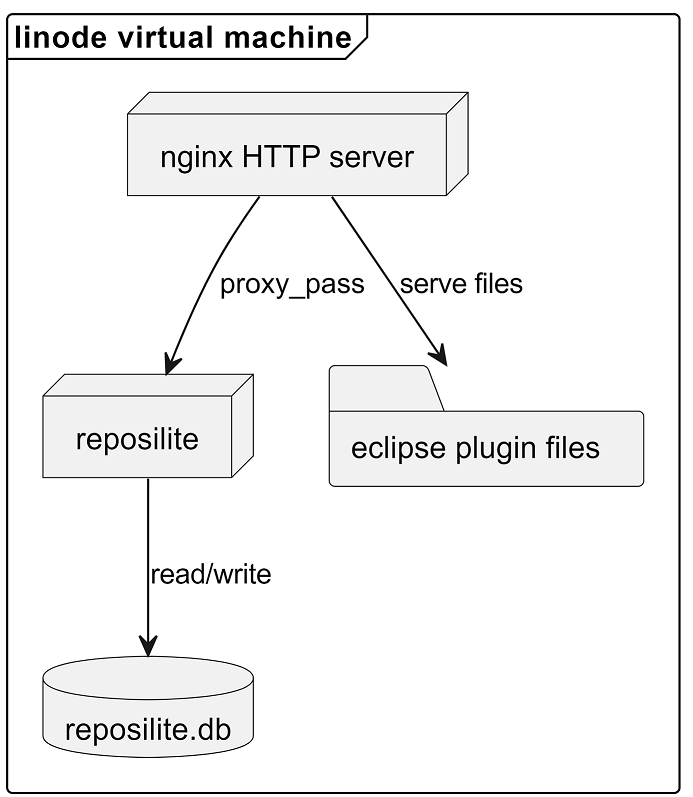
\includegraphics{ch3-images/deployment.png}
    \caption{Repository Hosting}
    \label{fig: Repository Hosting}
 \end{figure}

\begin{enumerate}
    \item I registered the domain ``languageslocalization.com" with the registrar ``GoDaddy".
    \item I created a virtual machine to host the sites ``maven.languageslocalization.com", and ``eclipse.languageslocalization.com". I used Linode as the cloud hosting provider. 
    \item I used Reposilite which is an open-source lightweight repository manager for Maven artifacts written in Java to host the Maven repository maven.languageslocalization.com. Moreover, I used nginx as a reverse proxy to Reposilite to provide \ac{SSL}/\ac{TLS} functionality.
    \item I used nginx to serve the static files generated by the plugin site project using the URL eclipse.languageslocalization.com.
    \item I used Certbot to configure, install, and renew the SSL/TLS certificate.
\end{enumerate}
\subsection{Plugin Installation}
To test the plugin, I created a \ac{VM} and installed Eclipse IDE to test all functionalities and features of the Eclipse Plugin. To install the plugin, a couple of steps must be done:

\begin{enumerate}
    \item After opening Eclipse, I must go to the help item in the menu bar and select ``Install New Software" as shown in the following figure:

    \begin{figure}[H]
        \centering
        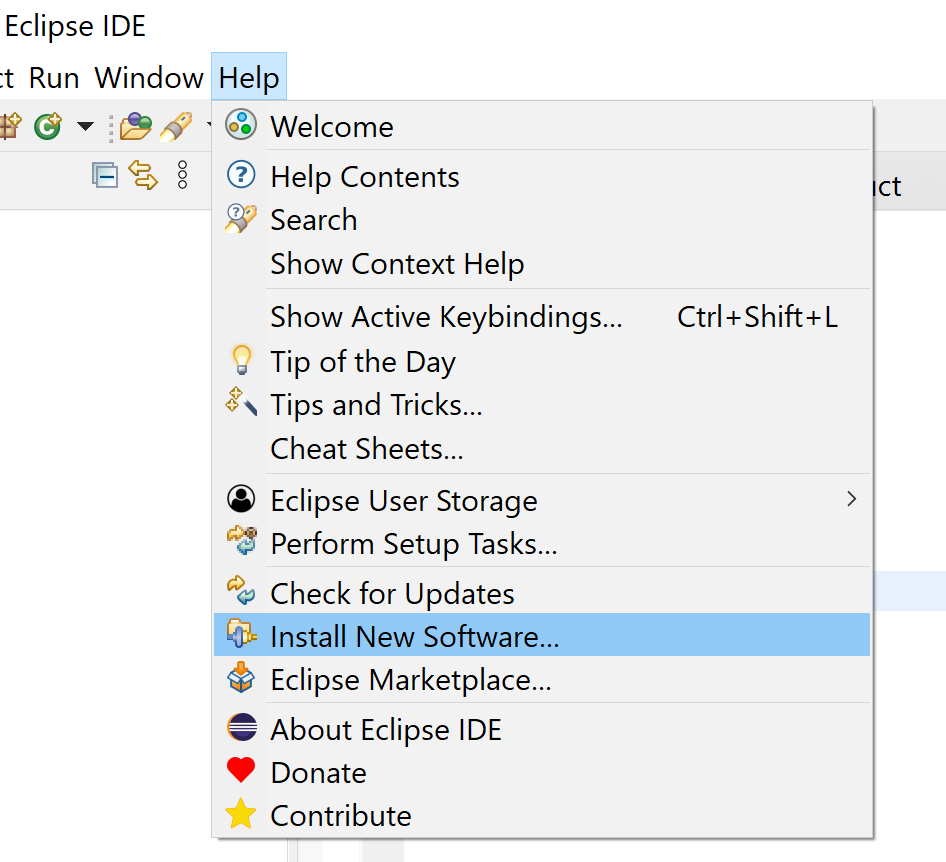
\includegraphics{ch3-images/installsoftware.png}
        \caption{Installing new software}
        \label{fig: Installing New Software}
    \end{figure}

    \item After selecting ``Install New Software", I must enter the \ac{URL} ``https://www.languageslocalization.com" to add my plugin repository as shown in the following figure:

    \begin{figure}[H]
        \centering
        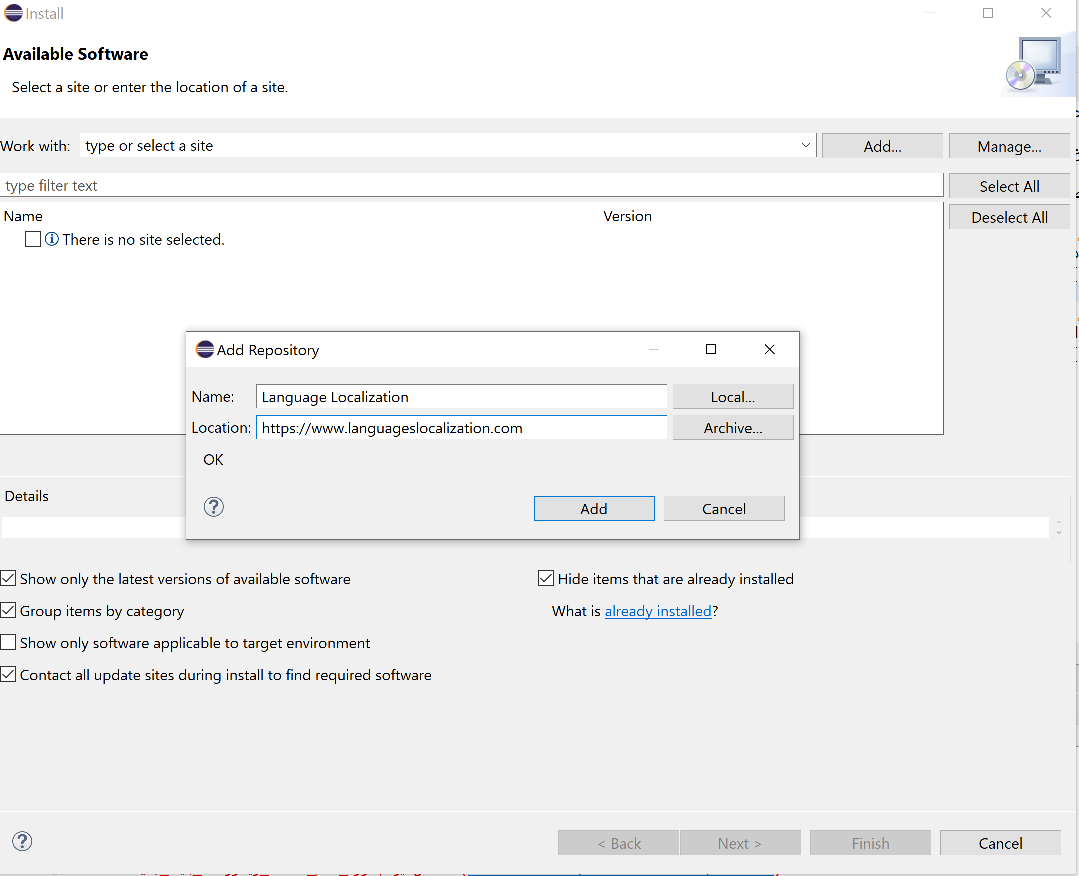
\includegraphics{ch3-images/addplugin.png}
        \caption{Adding plugin repository}
        \label{fig: Adding plugin repository}
    \end{figure}

    \item Finally, I must select my plugin and select ``Finish" to complete the installation and Eclipse will be restarted with my plugin added.
    
\end{enumerate}